%%%%%%%%%%%%%%%%%%%%%%%%%%%%%%%%%%%%%%%%%
% Beamer Presentation
% LaTeX Template
% Version 1.0 (10/11/12)
%
% This template has been downloaded from:
% http://www.LaTeXTemplates.com
%
% License:
% CC BY-NC-SA 3.0 (http://creativecommons.org/licenses/by-nc-sa/3.0/)
%
%%%%%%%%%%%%%%%%%%%%%%%%%%%%%%%%%%%%%%%%%

%----------------------------------------------------------------------------------------
%	PACKAGES AND THEMES
%----------------------------------------------------------------------------------------

\documentclass{beamer}

\mode<presentation> {

% The Beamer class comes with a number of default slide themes
% which change the colors and layouts of slides. Below this is a list
% of all the themes, uncomment each in turn to see what they look like.

%\usetheme{default}
%\usetheme{AnnArbor}
%\usetheme{Antibes}
%\usetheme{Bergen}
%\usetheme{Berkeley}
%\usetheme{Berlin}
%\usetheme{Boadilla}
%\usetheme{CambridgeUS}
%\usetheme{Copenhagen}
%\usetheme{Darmstadt}
%\usetheme{Dresden}
%\usetheme{Frankfurt}
%\usetheme{Goettingen}
%\usetheme{Hannover}
%\usetheme{Ilmenau}
%\usetheme{JuanLesPins}
%\usetheme{Luebeck}
\usetheme{Madrid}

\usepackage{listings} % Required for insertion of code
%\usetheme{Malmoe}
%\usetheme{Marburg}
%\usetheme{Montpellier}
%\usetheme{PaloAlto}
%\usetheme{Pittsburgh}
%\usetheme{Rochester}
%\usetheme{Singapore}
%\usetheme{Szeged}
%\usetheme{Warsaw}

% As well as themes, the Beamer class has a number of color themes
% for any slide theme. Uncomment each of these in turn to see how it
% changes the colors of your current slide theme.

%\usecolortheme{albatross}
%\usecolortheme{beaver}
%\usecolortheme{beetle}
%\usecolortheme{crane}
%\usecolortheme{dolphin}
%\usecolortheme{dove}
%\usecolortheme{fly}
%\usecolortheme{lily}
%\usecolortheme{orchid}
%\usecolortheme{rose}
%\usecolortheme{seagull}
%\usecolortheme{seahorse}
%\usecolortheme{whale}
%\usecolortheme{wolverine}

%\setbeamertemplate{footline} % To remove the footer line in all slides uncomment this line
%\setbeamertemplate{footline}[page number] % To replace the footer line in all slides with a simple slide count uncomment this line

%\setbeamertemplate{navigation symbols}{} % To remove the navigation symbols from the bottom of all slides uncomment this line
}

\usepackage{graphicx} % Allows including images
\usepackage{booktabs} % Allows the use of \toprule, \midrule and \bottomrule in tables
\usepackage{framed}

%----------------------------------------------------------------------------------------
%	TITLE PAGE
%----------------------------------------------------------------------------------------

\title[Introduzione]{MVC} % The short title appears at the bottom of every slide, the full title is only on the title page

\author{Claudio Menghi,  Srdan Krstic} % Your name
\institute[Deepse group] % Your institution as it will appear on the bottom of every slide, may be shorthand to save space
{
Politecnico di Milano \\ % Your institution for the title page
\medskip
\textit{menghi@elet.polimi.it,  srdan.krstic@polimi.it} % Your email address
}
\date{\today} % Date, can be changed to a custom date

\begin{document}

\begin{frame}
\titlepage % Print the title page as the first slide
\end{frame}

\begin{frame}
\frametitle{Overview} % Table of contents slide, comment this block out to remove it
\tableofcontents % Throughout your presentation, if you choose to use \section{} and \subsection{} commands, these will automatically be printed on this slide as an overview of your presentation
\end{frame}

%----------------------------------------------------------------------------------------
%	PRESENTATION SLIDES
%----------------------------------------------------------------------------------------

\begin{frame}
\frametitle{Commenti sul progetto}
\begin{figure}
\centering
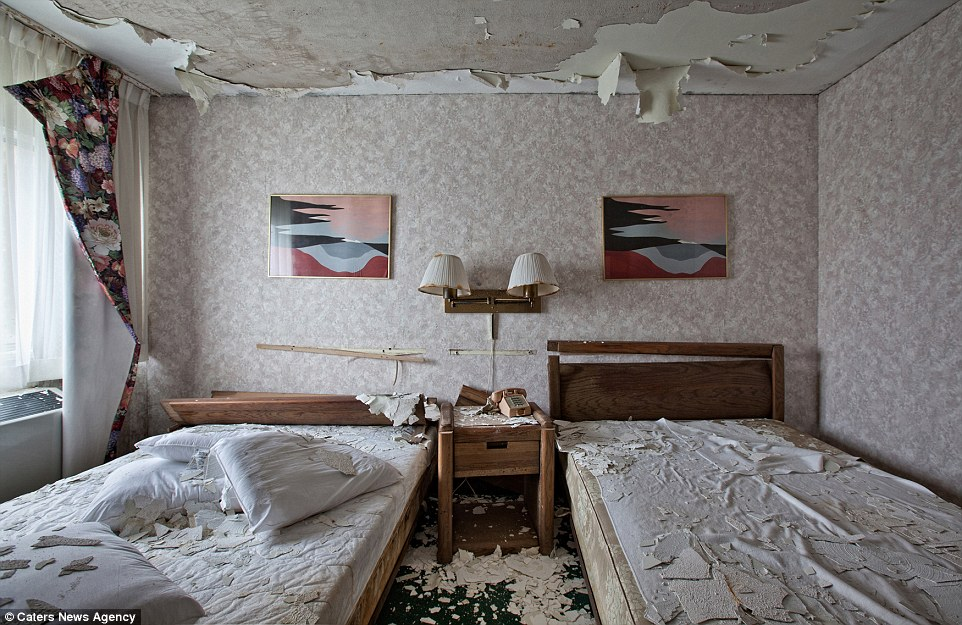
\includegraphics[width=0.5\textwidth]{Img/OrribleBedroom.jpg}
\end{figure}
\end{frame}

\begin{frame}
\frametitle{Commenti sul progetto}
\begin{figure}
\centering
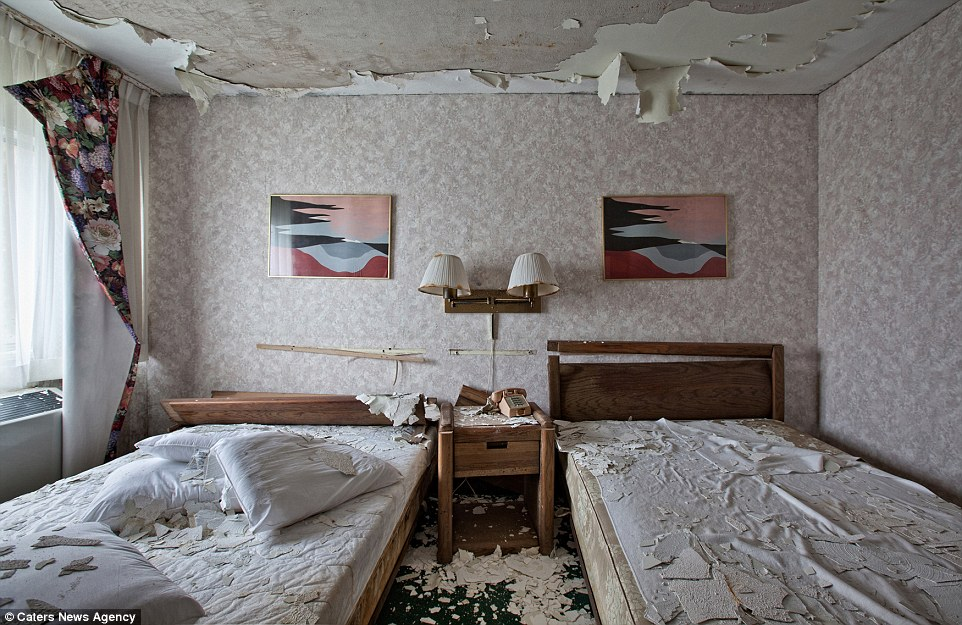
\includegraphics[width=0.5\textwidth]{Img/OrribleBedroom.jpg}
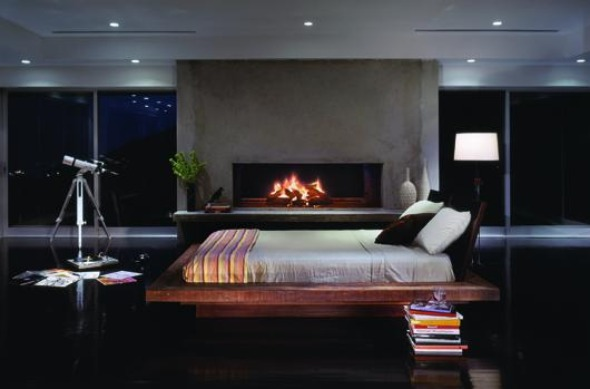
\includegraphics[width=0.5\textwidth]{Img/beedroom2.jpg}
\end{figure}
\end{frame}

\begin{frame}
\frametitle{Commenti discordanti}
\begin{figure}
\centering
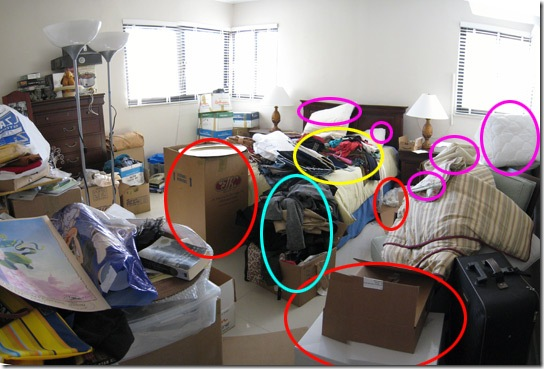
\includegraphics[width=0.5\textwidth]{Img/commenti1.jpg}
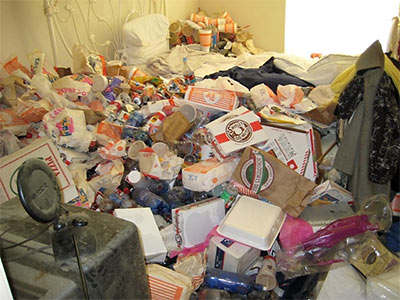
\includegraphics[width=0.5\textwidth]{Img/commenti2.jpg}
\end{figure}
\end{frame}


\begin{frame}
\frametitle{Situazione attuale}
\begin{itemize}
\item MOLTO MALE 20\% 
\item MEDI 60\% 
\item ALTI 20\% 
\item ECCELLENTI 0\% 
\end{itemize}
\end{frame}


\begin{frame}
\frametitle{Che cosa non va...}
\begin{figure}
\centering
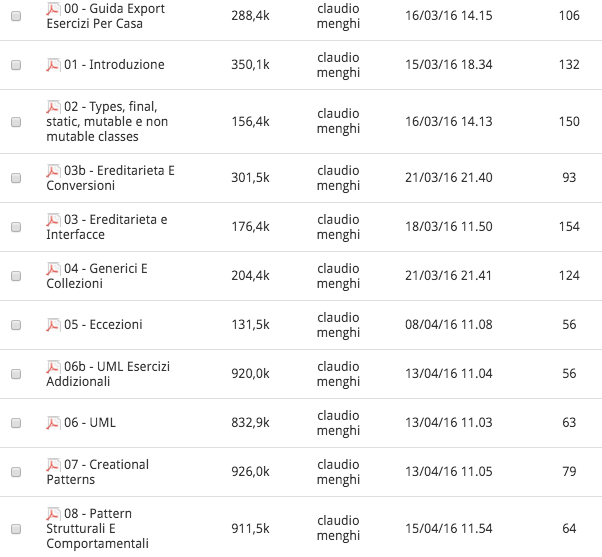
\includegraphics[width=0.5\textwidth]{Img/download.png}
\end{figure}
\end{frame}

\begin{frame}
\frametitle{Che cosa non va...}
Spero di non farle perdere tempo con la seguente spiegazione prolissa ma avendo il giorno libero domani io e il mio collega volevamo approfittarne per programmare per molte ore ma senza un modello fisso non possiamo proseguire
\end{frame}




\section{Design Principles}



\begin{frame}
\frametitle{Design Principles}
Open Close Principle
\begin{framed}
Le entit\`a del software (le classi, i moduli e le funzioni) devono essere \emph{aperte all'estensione} e \emph{chiuse alle modifiche}\\
\end{framed}
\end{frame}


\begin{frame}
\frametitle{Design Principles}
Open Close Principle
\begin{framed}
Le entit\`a del software (le classi, i moduli e le funzioni) devono essere \emph{aperte all'estensione} e \emph{chiuse alle modifiche}\\
\end{framed}
Sintomi di violazione 
\begin{itemize}
\item enumerations
\item primitive obsessions 
\end{itemize}
\begin{figure}
\centering
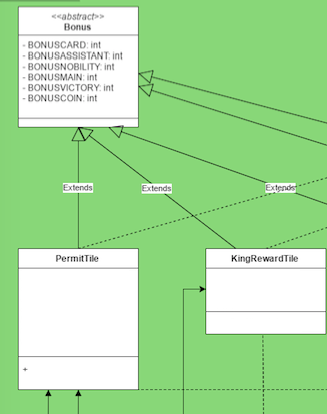
\includegraphics[width=0.3\textwidth]{Img/primitiveObsession.png}
\end{figure}
\end{frame}

\begin{frame}
\frametitle{Design Principles}
Open Close Principle
\begin{framed}
Le entit\`a del software (le classi, i moduli e le funzioni) devono essere \emph{aperte all'estensione} e \emph{chiuse alle modifiche}\\
\end{framed}
Sintomi di violazione 
\begin{itemize}
\item enumerations
\item primitive obsessions 
\end{itemize}
\begin{figure}
\centering
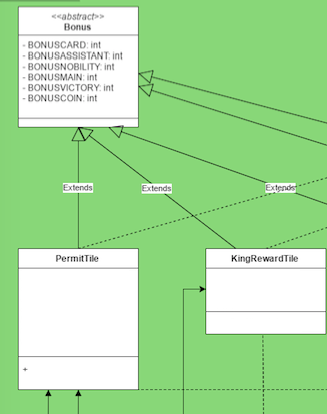
\includegraphics[width=0.3\textwidth]{Img/primitiveObsession.png}
\end{figure}
\end{frame}

\begin{frame}
\frametitle{Design Principles}
Open Close Principle
\begin{framed}
Le entit\`a del software (le classi, i moduli e le funzioni) devono essere \emph{aperte all'estensione} e \emph{chiuse alle modifiche}\\
\end{framed}
Sintomi di violazione 
\begin{itemize}
\item enumerations
\item primitive obsessions 
\end{itemize}
Serve davvero enum per MARE, MONTAGNA COLLINA? Si puo' fare meglio?
\end{frame}

\begin{frame}
\frametitle{Design Principles}
Dependency Inversion Principle
\begin{framed}
I moduli di alto livello non devono dipendere direttamente dai moduli di basso livello. Entrambi devono dipendere da delle astrazioni.
\end{framed}
Quando delle classi di alto livello devono accedere a delle risorse di basso livello (disco I/O etc..) \`e conveniente
\end{frame}


\begin{frame}
\frametitle{Design Principles}
Single Responsibility Principle
\begin{framed}
A class should have only one reason to change.
\end{framed}
Sintomi di violazione 
\begin{itemize}
\item classi con molti metodi
\end{itemize}

Scusi ma prof, per ogni classe l'unico attributo sarebbe solamente un singolo int

\end{frame}

\begin{frame}
\frametitle{Design Principles}
Liskov's Substitution Principle
\begin{framed}
Derived types must be completely substitutable for their base types.
\end{framed}

Sintomi di violazione 
\begin{itemize}
\item quando estendete invece che estendere riducete il comportamento
\end{itemize}
\end{frame}


%----------------------------------------------------------------------------------------
%	PRESENTATION SLIDES
%----------------------------------------------------------------------------------------



\section{MVC}
\begin{frame}
\frametitle{MVC}
Il model view controller viene inzialmente creato come una soluzione al problema di fornire agli utenti il controllo delle loro informazioni quando visualizzate su perspectives multipli, in particolare quando si devono trattare data-set di grandi dimensioni.
\begin{figure}
\centering
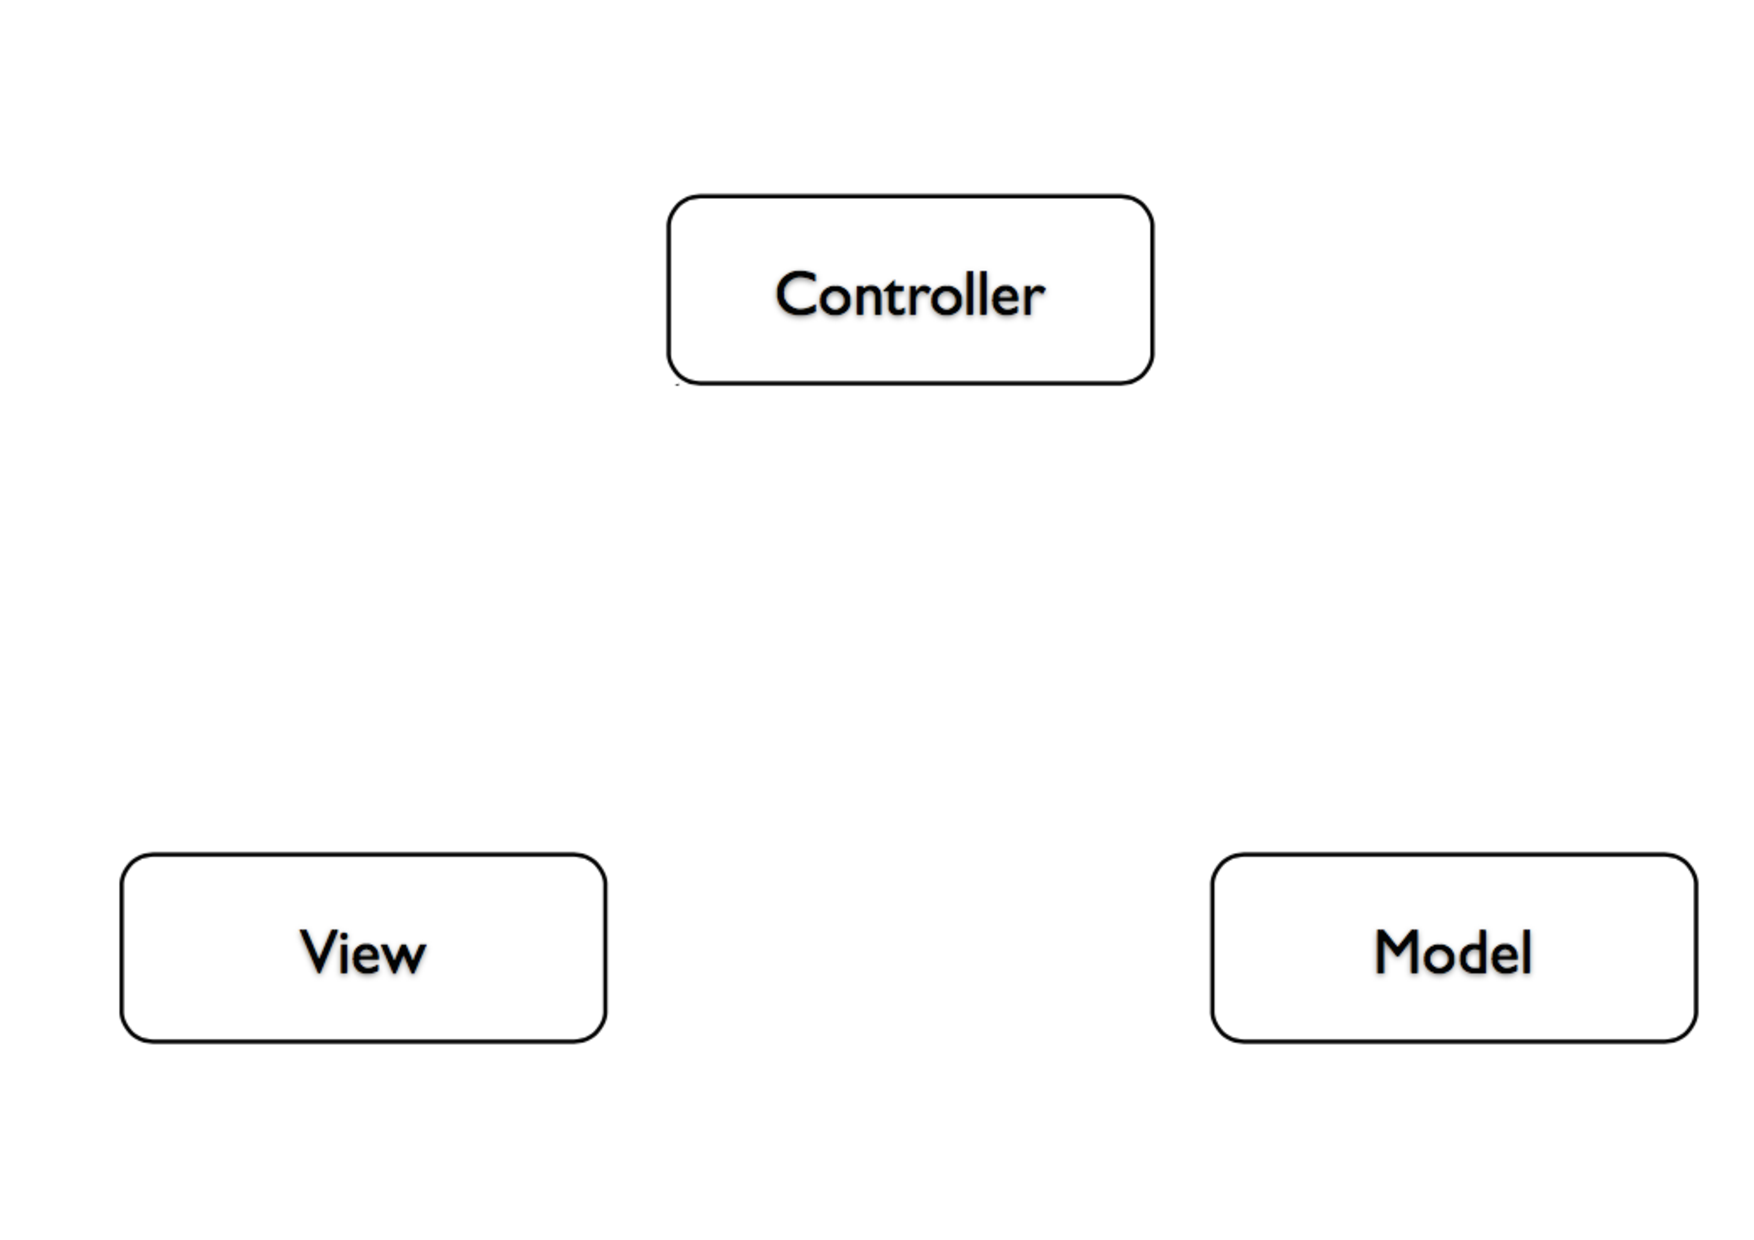
\includegraphics[width=0.5\textwidth]{Img/MVC1.pdf}
\end{figure}
\end{frame}

\begin{frame}
\frametitle{MVC}
\begin{figure}
\centering
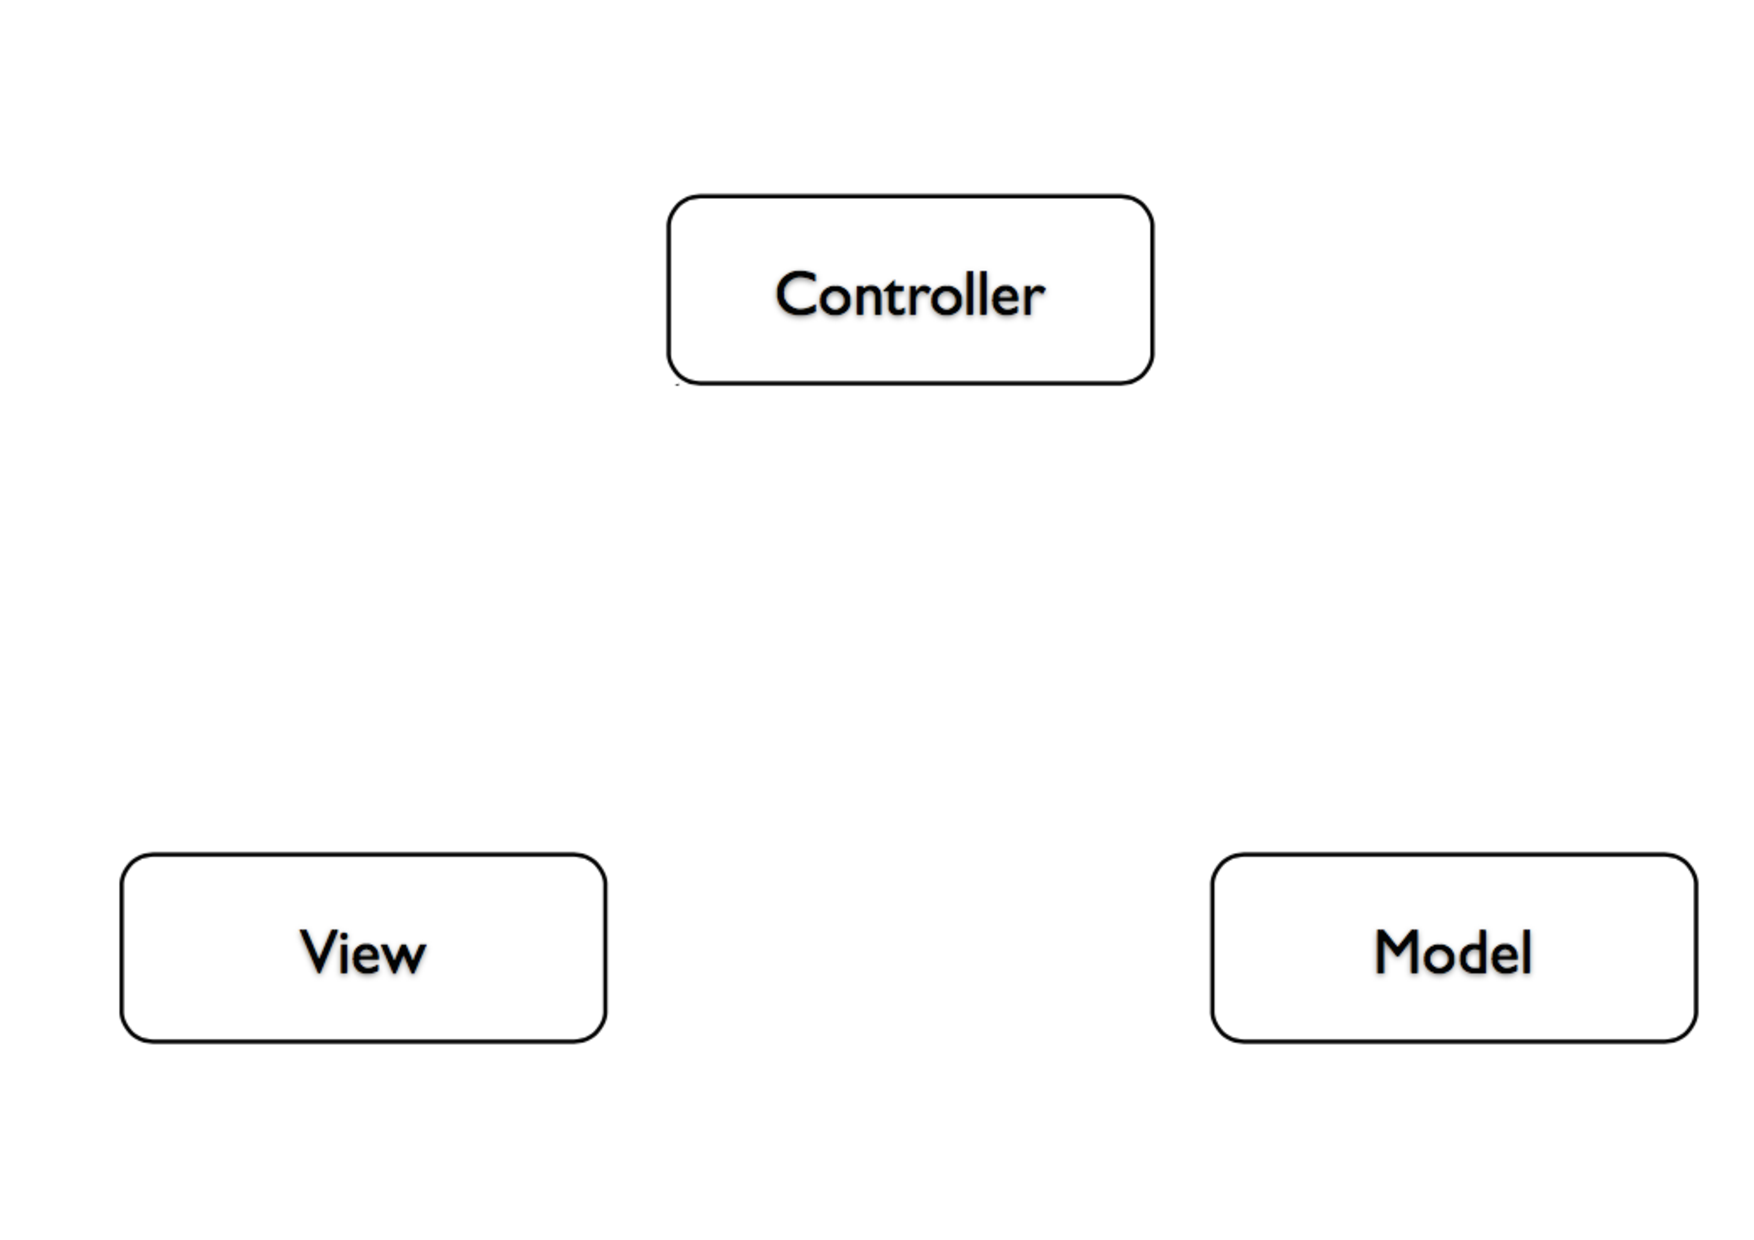
\includegraphics[width=0.5\textwidth]{Img/MVC1.pdf}
\end{figure}
\centering
\begin{itemize}
\item \emph{Model}: \`e una rappresentazione astratta del sistema che si desidera modellare. 
\begin{itemize}
\item Il modello include i dati assieme ai metodi (logica) necessari per processare questi dati. 
\item Il modello non include nessuna informazione di \emph{come} i dati sono visualizzati
\end{itemize}
\end{itemize}
\end{frame}

\begin{frame}
\frametitle{MVC}
\begin{figure}
\centering
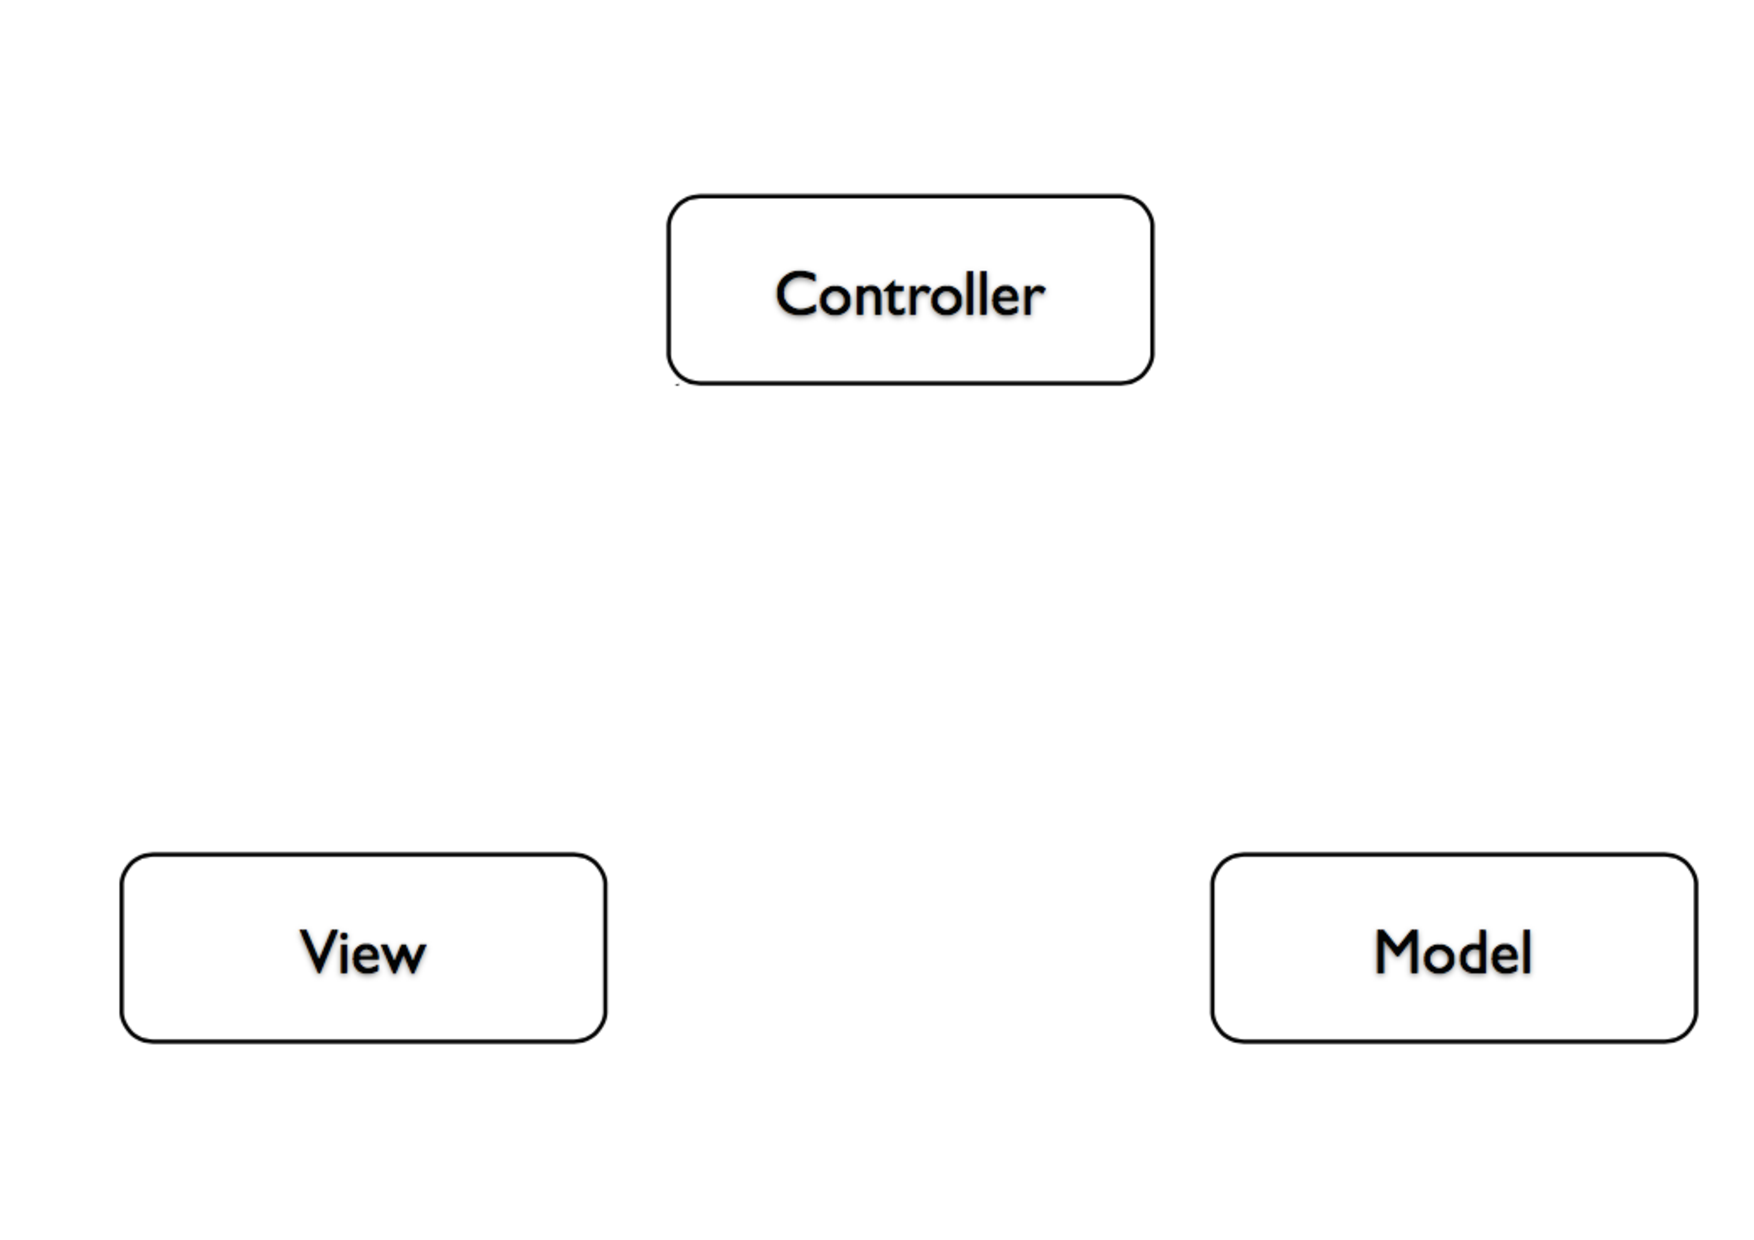
\includegraphics[width=0.5\textwidth]{Img/MVC1.pdf}
\end{figure}
\begin{itemize}
\item \emph{View} (Interface): viene utilizzata per mostrare un modello. In genere,  un  modello pu\`o essere mostrato da pi\`u Views, ogni view \`e capace di mostrare una o pi\`u rappresentazione del modello (esempio una rappresentazione su schermo o cartacea). La view consente di:
\begin{itemize}
\item mostrare dei dati a un utente
\item essere aggiornata quando il modello cambia
\end{itemize}
\end{itemize}
\end{frame}



\begin{frame}
\frametitle{MVC}
\begin{figure}
\centering
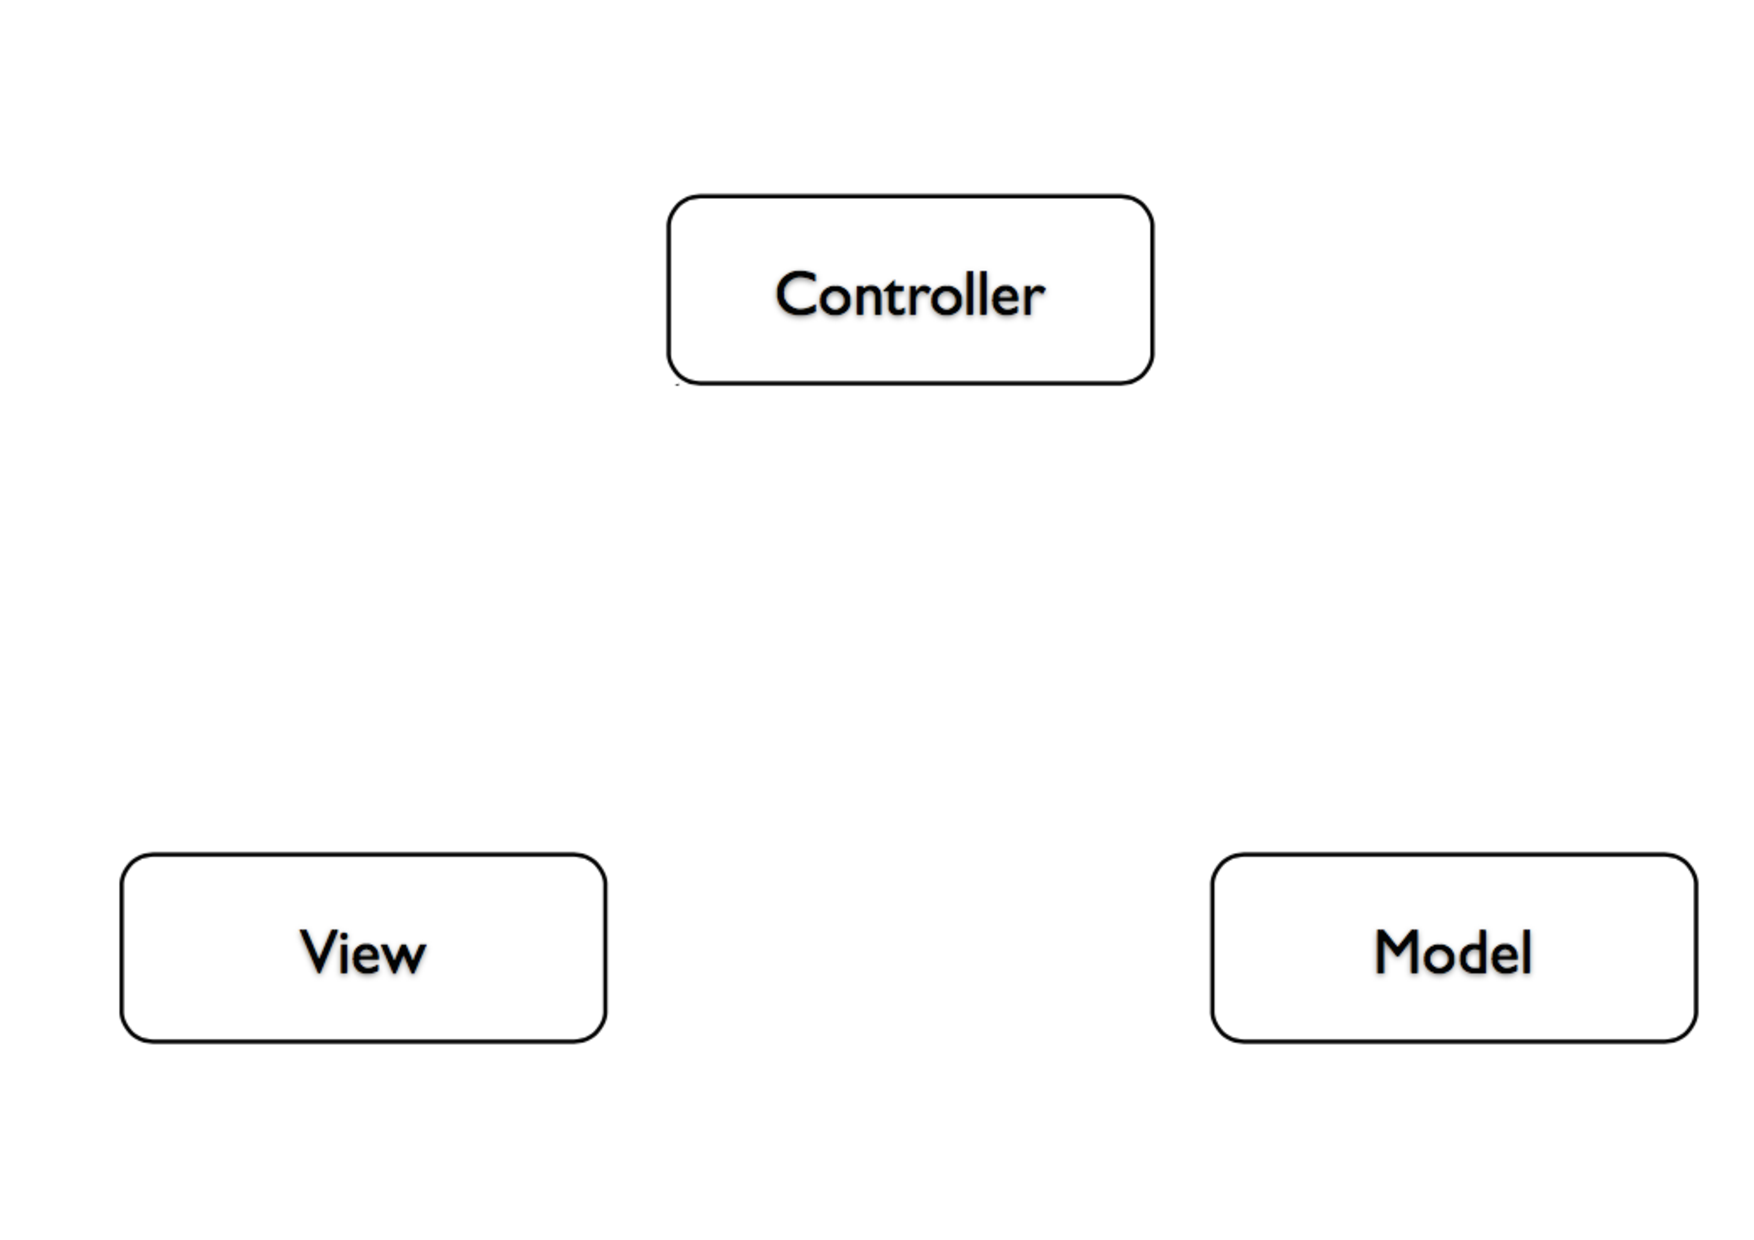
\includegraphics[width=0.5\textwidth]{Img/MVC1.pdf}
\end{figure}
\begin{itemize}
\item \emph{Controller} (Coordinator): riceve gli input dalla view e li trasforma in azioni che il modello pu\`o eseguire. Delle azioni potrebbero essere il click su un bottone nel caso di una GUI o delle richieste GET e POST in una applicazione web. Il controller in alcuni casi potrebbe selezionare nuove view, per esempio nel caso delle richieste HTTP.
\end{itemize}
\end{frame}


\begin{frame}
\frametitle{Interazione ``classica"}
Trygve Reenskaug nel 1979
\begin{figure}
\centering
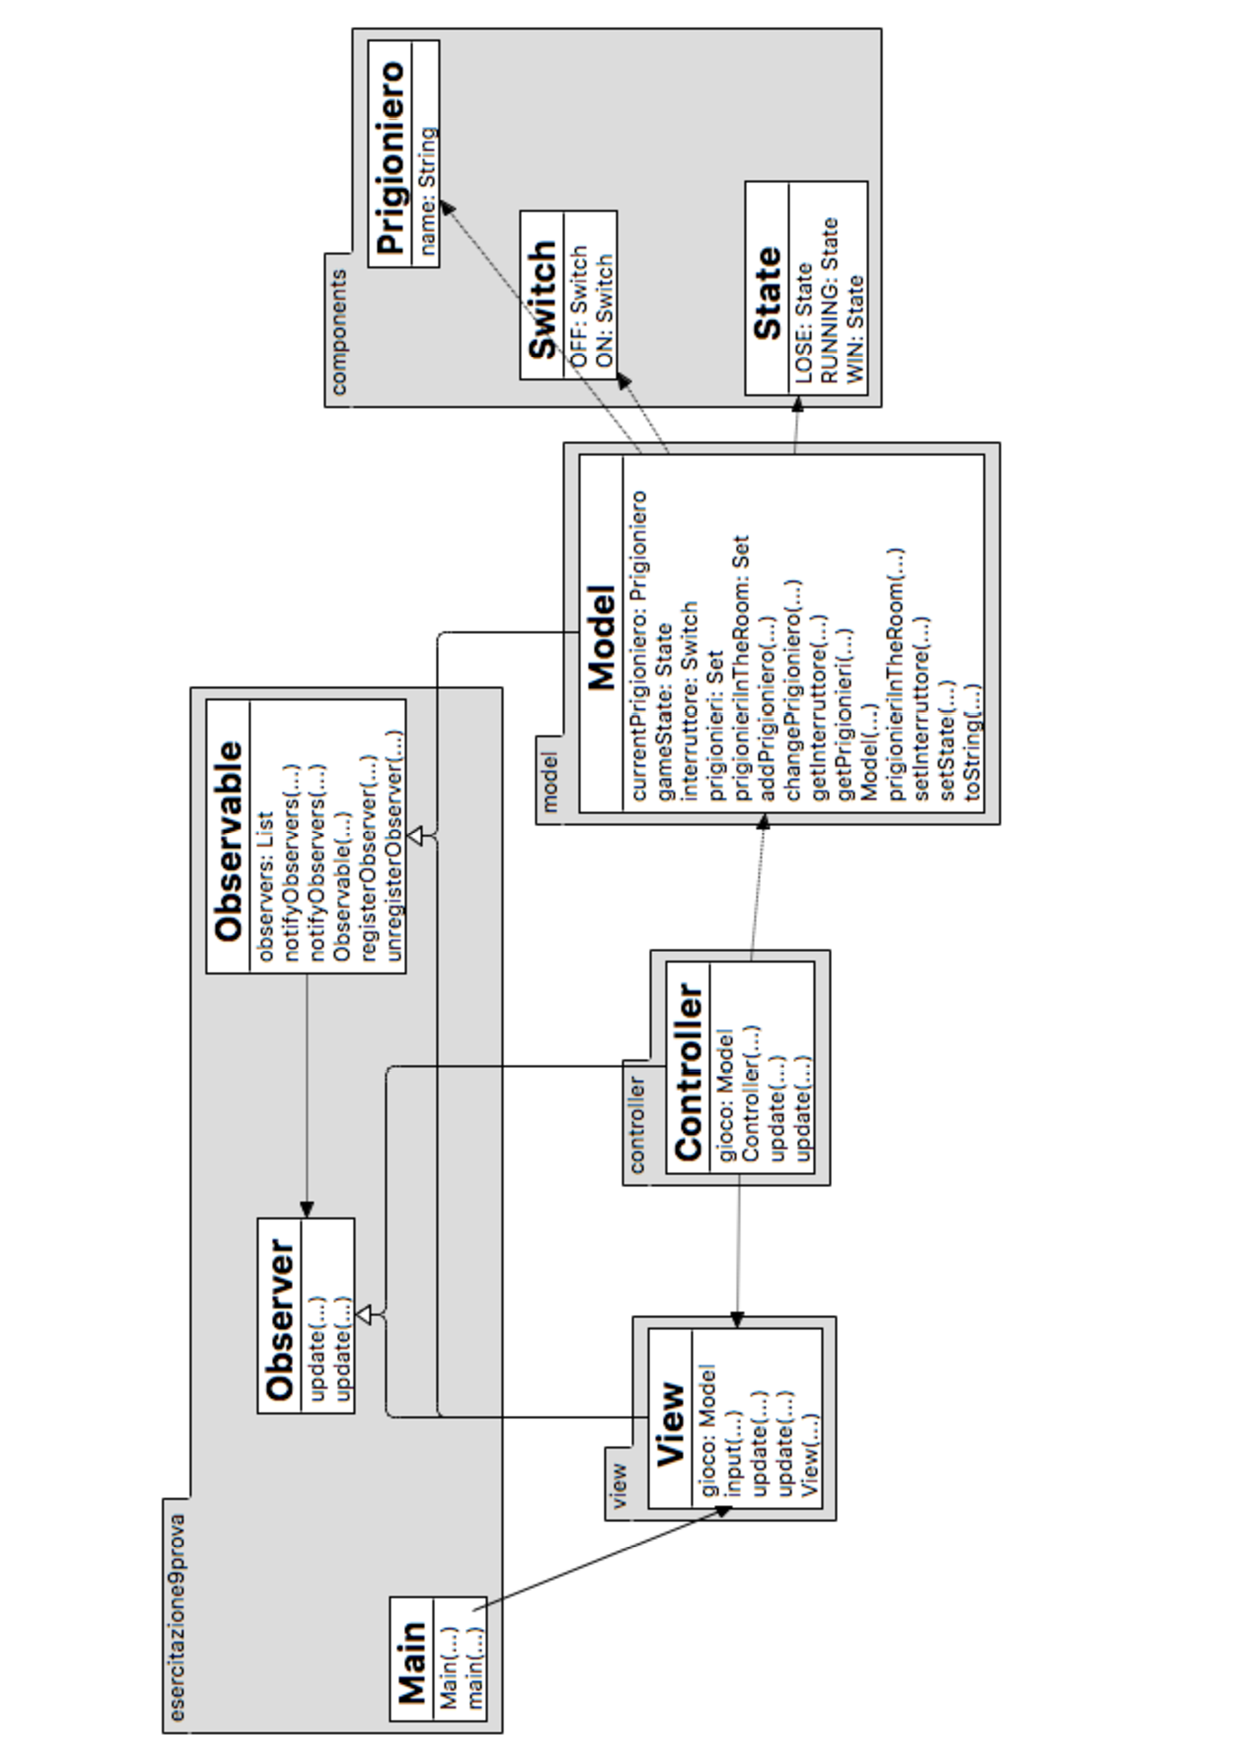
\includegraphics[width=0.5\textwidth]{Img/MVC.pdf}
\end{figure}
 La \emph{view} osserva (pattern observer o listener) il modello. Ogni cambiamento al al modello viene propagato come una notifica che la view riceve. Nota il modello non \`e direttamente consapevole di chi osserva, semplicemente manda un messaggio agli ascoltatori.
\end{frame}

\begin{frame}
\frametitle{MVC}
\begin{figure}
\centering
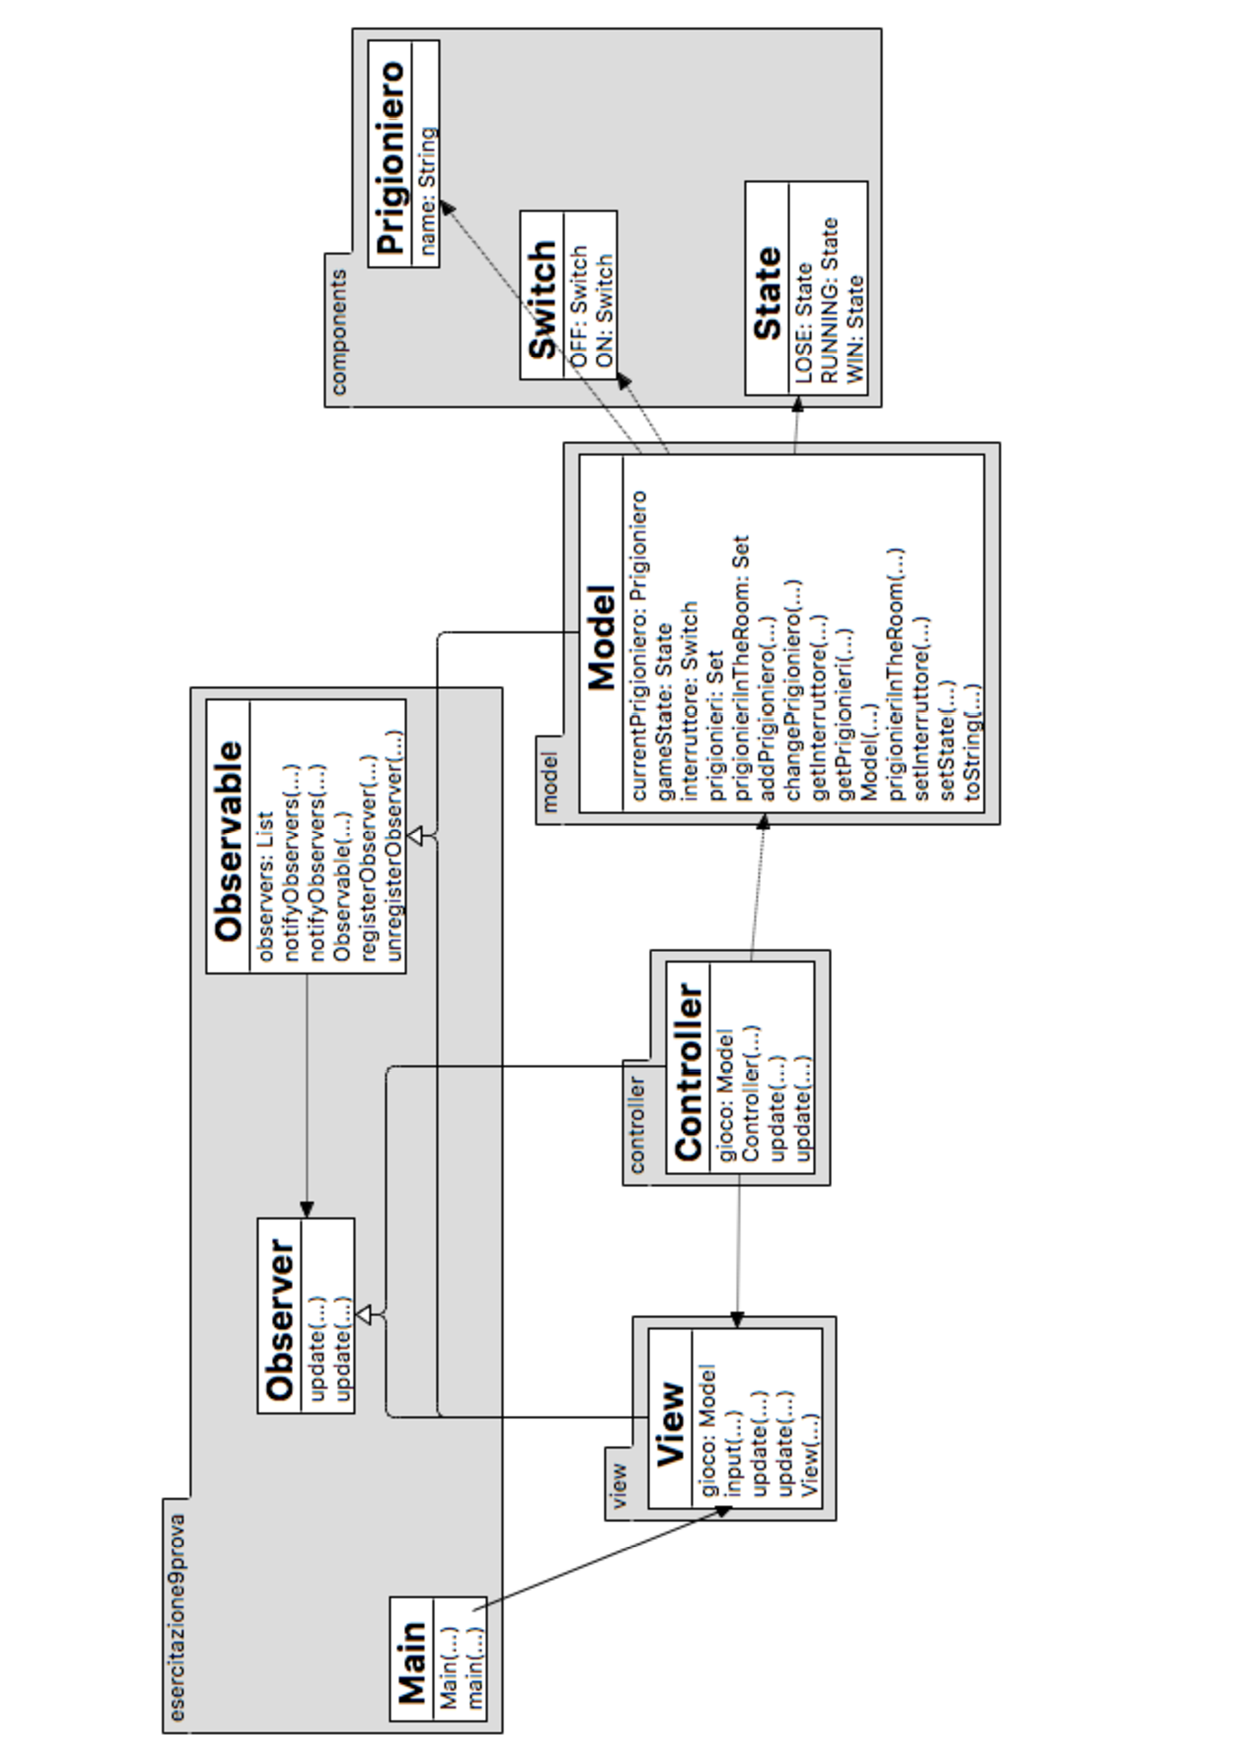
\includegraphics[width=0.5\textwidth]{Img/MVC.pdf}
\end{figure}
\begin{itemize}
\item \emph{push model} la view si registra al modello e aspetta notifiche
\item \emph{pull model} la view \`e responsabile di eseguire delle query sul modello quando deve aggiornare la sua visualizzazione
\end{itemize}
\end{frame}

\begin{frame}
\frametitle{Interazione ``classica"}
\begin{figure}
\centering
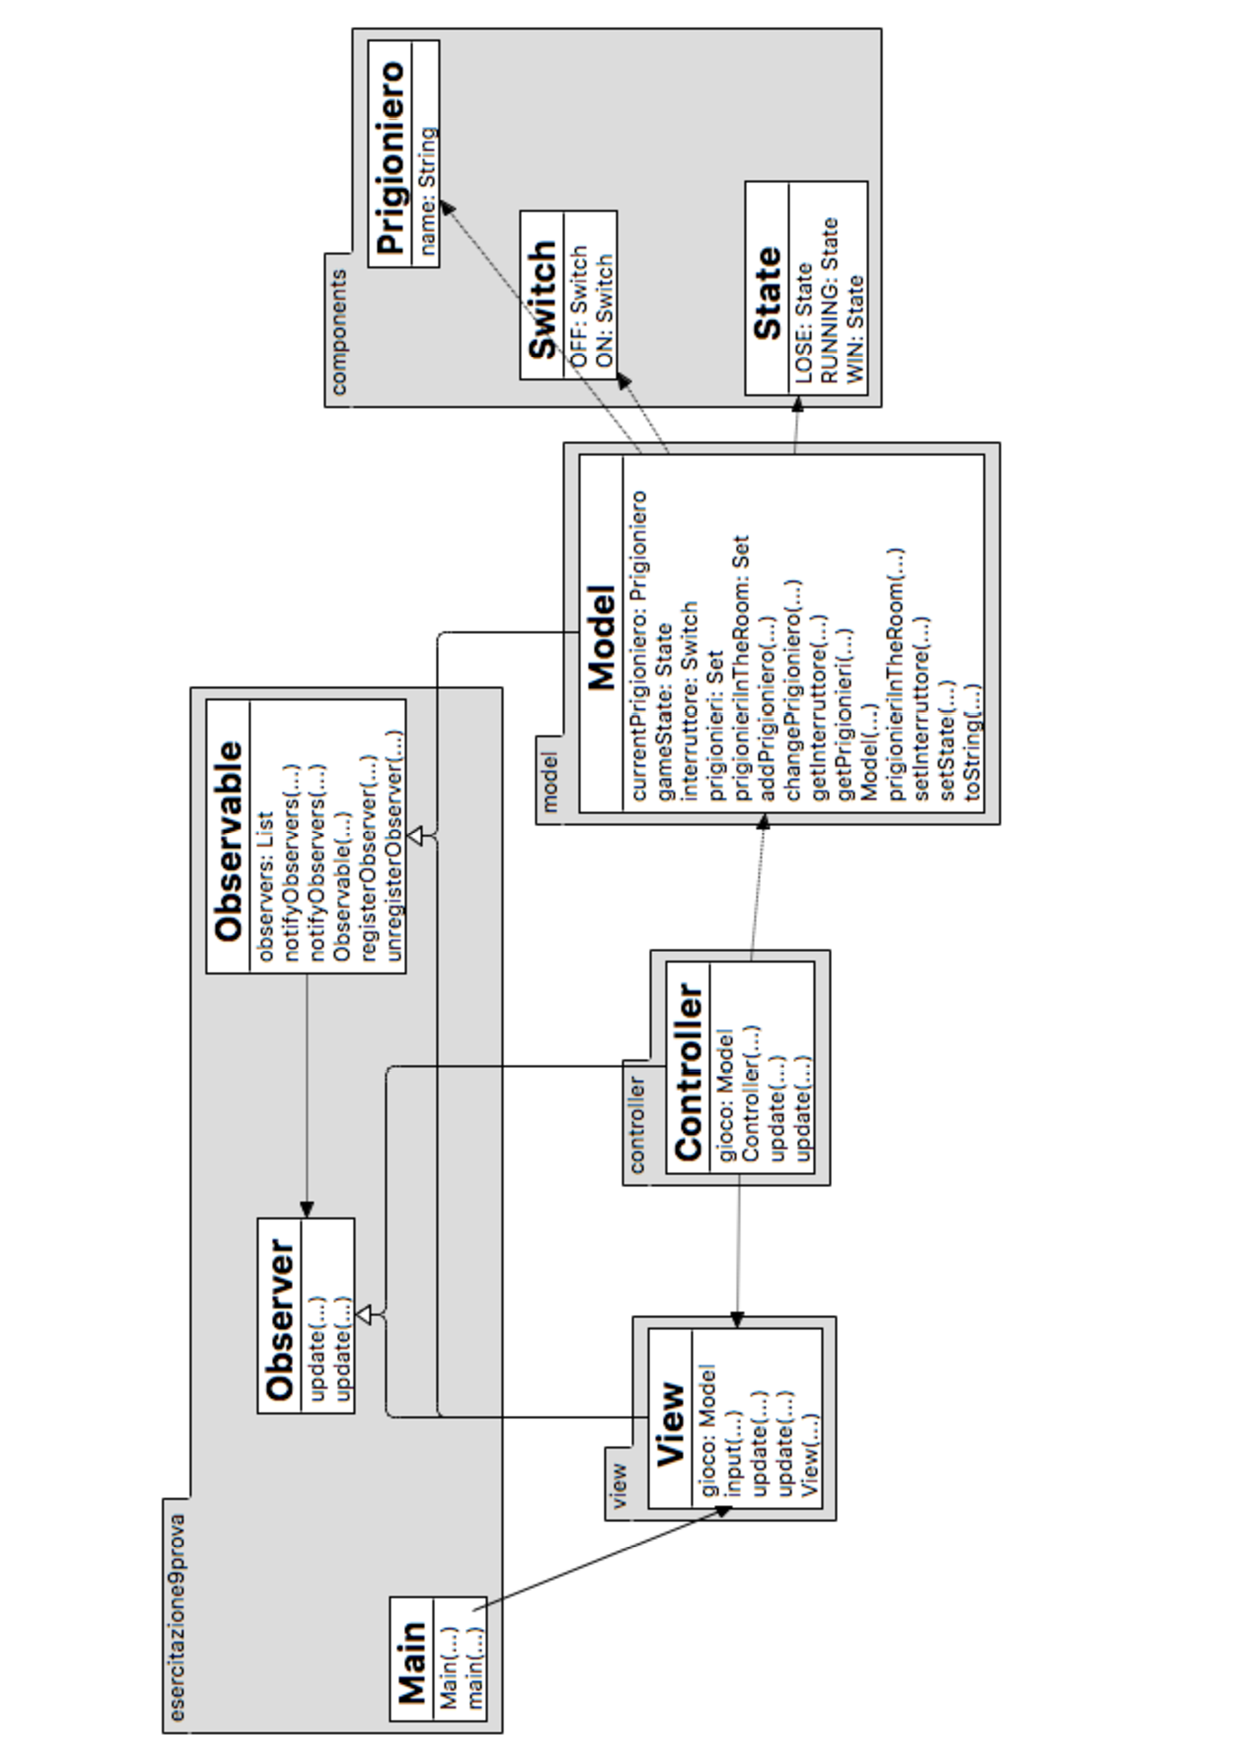
\includegraphics[width=0.5\textwidth]{Img/MVC.pdf}
\end{figure}
Il \emph{controller} \`e azionato dalla view (o da una sua logica interna). Quando un azione viene eseguita sulla view, una notifica viene mandata al controller. Il controller osserva la view (mediante un osservatore o un listener). Il controller conosce il modello sottostante. Quando un azione viene eseguita sulla view (un comando chiamato sull'interfaccia del server), l'azione viene segnalata al controller, il controller accede al modello e lo aggiorna in relazione all'azione dell'utente.
\end{frame}

\begin{frame}
\frametitle{Interazione ``classica"}
\begin{figure}
\centering
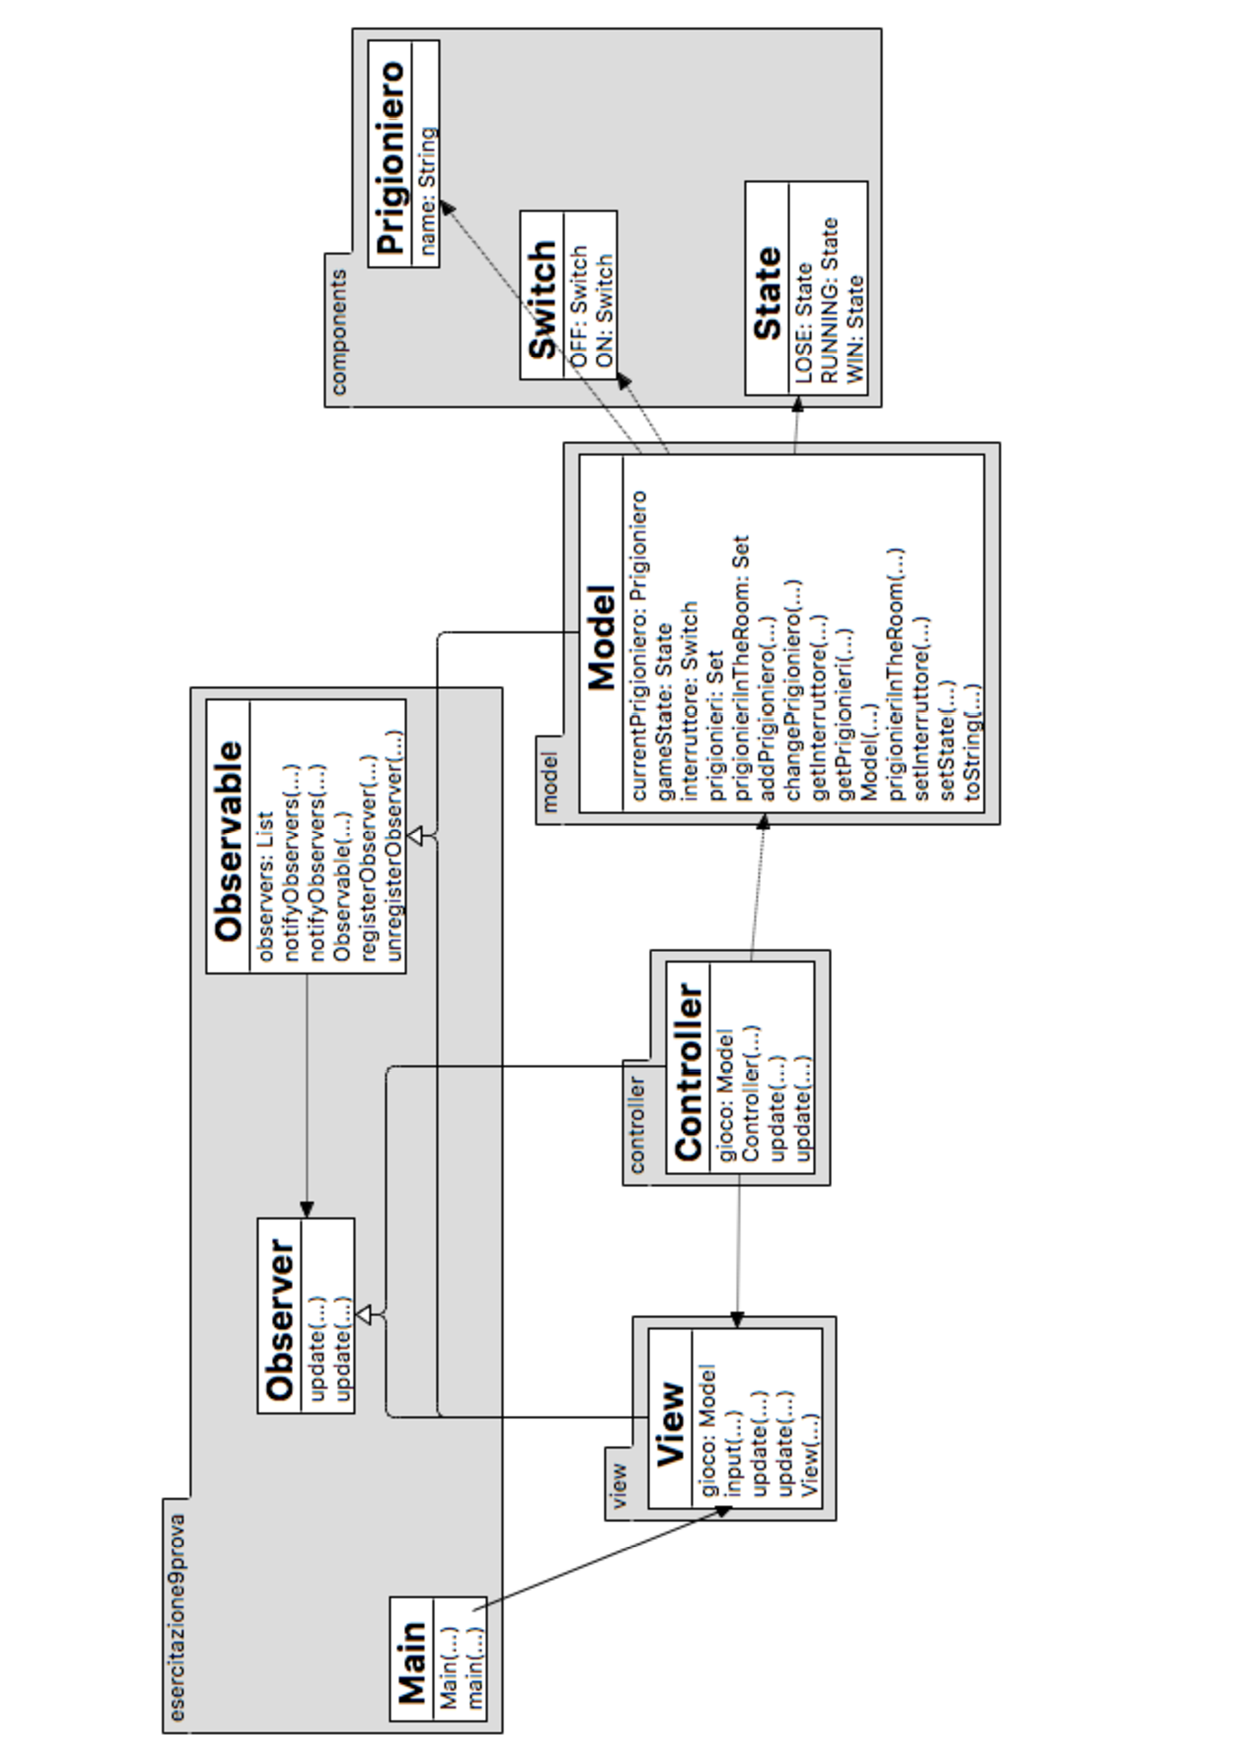
\includegraphics[width=0.5\textwidth]{Img/MVC.pdf}
\end{figure}
Il \emph{controller} \`e azionato dalla view (o da una sua logica interna). Quando un azione viene eseguita sulla view, una notifica viene mandata al controller. Il controller osserva la view (mediante un osservatore o un listener). Il controller conosce il modello sottostante. Quando un azione viene eseguita sulla view (un comando chiamato sull'interfaccia del server), l'azione viene segnalata al controller, il controller accede al modello e lo aggiorna in relazione all'azione dell'utente.
\end{frame}

\begin{frame}
\frametitle{Interazione Cocoa}
\begin{figure}
\centering
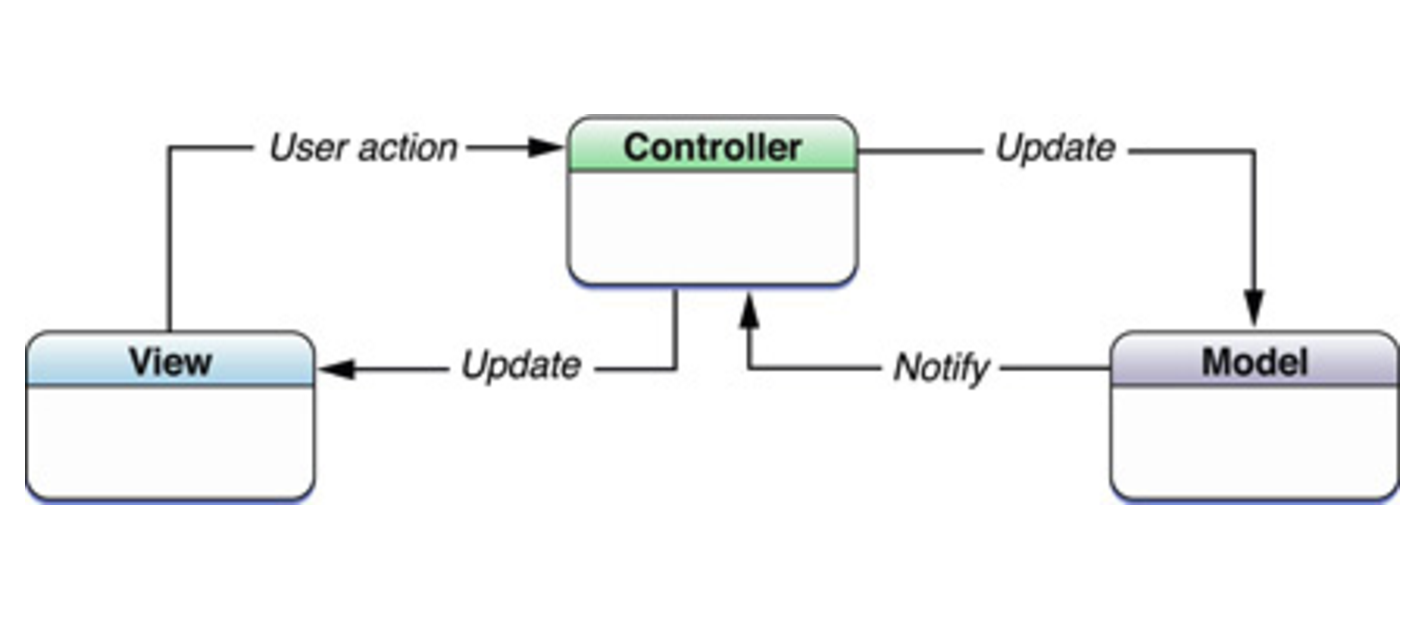
\includegraphics[width=0.7\textwidth]{Img/MVCCocoa.pdf}
\end{figure}
\end{frame}


\begin{frame}
\frametitle{MVC Client/Server}
In un architettura client/server l'MVC pu\`o essere visto a diversi livelli di astrazione a seconda della granularit\`a con cui si affronta il problema. Se si considera ``l'applicazione finale" la view rappresenta l'interfaccia con cui il client (utenti) interagisce. In questo contesto esistono due approcci:
\begin{itemize}
\item \emph{server-side} MVC: \`e il caso in cui model, view e controller sono eseguiti sul sever. \`E per esempio il caso delle pagine HTML (View)
che vengono generate sul server
\item \emph{client-side} MVC: \`e il caso in cui model e controller sono posti sul client. \`E il caso per esempio delle applicazioni per tablet.
\end{itemize}

Se invece consideriamo come ``granularit\`a" il server, i nostri client (utenti) sono le persone che useranno le API, ovvero le interfacce della nostra applicazione (View) che esponiamo, il controllore \`e il coordinatore che gestisce l'interazione tra le view e il modello che contiene lo stato del gioco. 
\end{frame}

\begin{frame}
\frametitle{MVC Client/Server}
Gestire il seguente gioco:
Dei carcerati sono in una prigione. I poliziotti della prigione decidono di salvare i carcerati se dimostrano una capacit\`a collaborativa e una certa attitudine nel risolvere problemi. I prigionieri vengono lasciati nel cortile della prigione per un determinato tempo al fine di accordarsi relativamente a una strategia per salvarsi. Dal giorno seguente in poi un prigioniero alla volta verr\`a fatto entrare in una cella $t$ contenente un interruttore.
Un prigioniero pu\`o  entrare pi\`u volte nella cella prima che un altro prigioniero entri e ad intervalli di tempo non prefissati. L'interruttore pu\`o essere in due stati ON e OFF. Ogni prigionierio pu\`o muovere l'interruttore da ON a OFF e viceversa o lasciarlo nello stato  attuale. Tra un prigioniero e l'altro l'interruttore non viene toccato dai poliziotti. L'unica informazione che si conosce \`e che l'interruttore \`e inizialmente a OFF. Il gioco continua finch\`e uno dei prigionieri dice: ``ogni prigioniero \`e stato nella cella prima di me almeno una volta". Se \`e corretto tutti i prigionieri sono liberati altrimenti vengono uccisi.
\end{frame}



%----------------------------------------------------------------------------------------

\end{document} 